%
%   Managing input data
%
\subsection{Managing input data} \label{subsec:RNN}
As discussed in the introduction, Section~\ref{sec:Introduction}, the purpose of the article is to analyse several different RNN models, measure the performance, and determine the most promising direction for further enhancing Neural Network models' integration into an embedded device.
Although the perfect replication was impossible due to a lack of details and actual battery data used by different authors, all models were implemented based on the provided information.
All missing aspects were assumed based on ML's standard methods at the time of their writing.
Summarising Table~\ref{tab:review} and Literature Review, Table~\ref{tab:experiment} compiles models, which will be evaluated in this work.
It provides details of 7 different implementations, which vary in their structure and learning process but share the same training, validation, testing and performance measurement procedures.
\begin{center}
    \begin{table}[h]
    \caption{Testing models summary.}
    \label{tab:experiment}
\begin{tabular}{p{0.4cm}|p{3.4cm}|p{1.3cm}|p{1.0cm}|p{1.2cm}|p{1.5cm}|p{1.5cm}|p{3.0cm}}
    \hline
    \multirow{2}{ 4em }{№} &
    \multirow{2}{ 4em }{Structure \& Cells} &
    \multirow{2}{ 4em }{State$-$ } &
    \multicolumn{4}{ c|}{Optimiser Learning Rate} &
    \multirow{2}{ 4em }{Extension} \\
    \cline{4-7}
      &                       &         & Adam  & Nadam & SGDw/M & AdaMax &           \\
    \hline
    1 & 1 $\times$ LSTM (500) & $-$less & 0.001 &       &        &        &           \\
    2 & 1 $\times$ GRU (560)  & $-$less &       & 0.001 &        & 0.0005 & Ensemble  \\
    3 & 1 $\times$ LSTM (520) & $-$less & 0.001 &       &        &        & Attention \\
    4 & 2 $\times$ GRU (64)   & $-$full &       &       & 0.01   &        & Momentum (0.8)\\
    5 & 4 $\times$ GRU (64)   & $-$full & 0.001 &       &        &        &           \\
    6 & 1 $\times$ GRU (500)  & $-$less & 0.001 &       &        &        & Robust (RoAdam)\\
    \hline
\end{tabular}
    \end{table}
\end{center}

%
%
The structure and cell type define the number of layers of particular cell types with the total number of neurons evenly shared across layers.
The statefulness parameter describes the model ability to preserve its' current state for the next set of input parameters.
Based on that, the input amount of sample becomes flexible by the requirement of adding only a single sample at a time upon their arrival, instead than wait until the fixed amount has arrived.
The optimiser selection was based on the derivative calculation algorithms only.
Other alternatives, like differential evolution, are beyond the scope of research.
Extention defines the specific detail of the model, which distinguish it against the others.

%
%
Thus the specifics of each algorithmic aspect will be defined in the following: 2.1,2.2,2.3
\begin{itemize}
    \item Data shape for each state type
    \item Model structure and difference between GRU and LSTM
    \item Each optimisation algorithm and hyper-parameters selection
\end{itemize}

%
%
\subsection{Dataset description and generator} \label{subsec:dataset}
Recurrent Neural Network is a subclass of NN, which has proven effective in weather or stock prices forecasting.
This method learns by recognising a pattern within sequential data input, thus predicting the future outcome.
It makes the following approach applicable to almost any type of time series dependant problem~\cite{anton_battery_2013}.
Classical RNN consists primarily of three layers, represented in Figure~\ref{fig:RNN-structure}.
The Input and Output Layers defined by the two vectors or matrices.
The general description of a single input X and an output Y samples represented by Equations~\ref{eq:xy-matrix}.
$V, I, T, SoC$ represent Voltage (V), Current (A), Temperature (\textdegree{}C) as input features, and percentage of State of Charge (between 0 and 1) as output.
All samples are equally time distributed, and the t represents the number of input time steps at a time.
\begin{equation}
    \textbf{X} \left (n  \right ) = 
    \begin{Bmatrix}
        V \left (0  \right ) & V \left (1  \right ) & ... & V \left (t  \right )\\ 
        I \left (0  \right ) & I \left (1  \right ) & ... & I \left (t  \right )\\ 
        T \left (0  \right ) & T \left (1  \right ) & ... & T \left (t  \right )\\
    \end{Bmatrix}
    \\ \textbf{Y} \left (n  \right ) = 
    \begin{Bmatrix}
        SoC \left (t  \right ) 
    \end{Bmatrix}
\label{eq:xy-matrix}
\end{equation}

%
%
For dataset generation of training and testing purposes, data is combined in a 3-dimensional matrix using windowing techniques as per Figure~\ref{fig:Windowing}, where $s$ represents the step between each window, less than the number of input time steps.
The most optimum size of the windows for stateless models, obtained by Chemali et al.~\cite{Chemali2017}, will be 500 samples.
Any more significant matrices will lead to an increase in computation time but an insignificant difference in performance.
All stateful models used the same windowing technique to keep data generation simple but with a sample size of 1.
The state reset for stateful models happens at the end of every dataset, allowing a batching mechanism to speed up the training process.
For example, 12 datasets of discharge process with similar Voltage, Current and the State of Charge, but different temperatures at a time $t$ can be treated as a single batch.
The statefulness of a model preserves the state at index $i$ to the same index in the next batch [ref to the document will not hurt].
%%%
% For the process of training for Stateful models speeding up, all data can be separated by batches \textit{b}, for each batch representing a different temperature category, creating a 4-dimensional matrix.
% \textit{f} defines the number of features as per Voltage, Current and Temperature.
% \textit{b} and \textit{s} were kept as the size of 1 for all scenarios to minimise resource consumption and simplify performance validation.
% Equation~\ref{eq:XY-shape} represent the final shape for Input data.
% The output shape for both Stateful and Stateless models remains the same.
% \begin{equation}
%     \begin{split}
%         X_{shape} = (n, b, t, f) & => (n, t, f) - Stateless \\
%                                  & => (n, 1, f) - Stateful \\
%         Y_{shape} = (n, b, 1) \ \ &=> (n, 1)
%     \end{split}
%     \label{eq:XY-shape}
% \end{equation}
%One of the first methods of SoC Estimation by Chemali \textit{et al.}~\cite{Chemali2017} proved that 500 input time-steps produced the most efficient results, any further grow made insignificant impact.
%The same value used in this article. \\

%
%
The value of SoC has been calculated from the difference between charge and discharge capacity.
Values were rounded to 2 decimal places and kept in the range of 0 and 1 using min-max normalisation to reduce error in estimation.
Since there is no way to directly obtain the battery's accurate charge practically during a run, output SoC excluded from the time-series model's input feature, unlike in any classic examples of usage Time-Series estimations.
The trainable model has to distribute weights across inputs and still develop a charge's close estimate.
All input samples were taken through normalisation by the mean and standard deviation across all input files with the same values, simplifying model weights acquiring and speeding up the training process.
It is important to note that the normalisation values of mean and standard deviation from a training dataset are applied to both validation and testings sets.

%
%
The training process conducted through all datasets for a single battery testing profile and validated on a single cycle (less or around 20\% of the entire set).
Final tests for a model performance conducted against an entire set of two remaining profiles separately.
\begin{figure}[htbp]
    \centering
    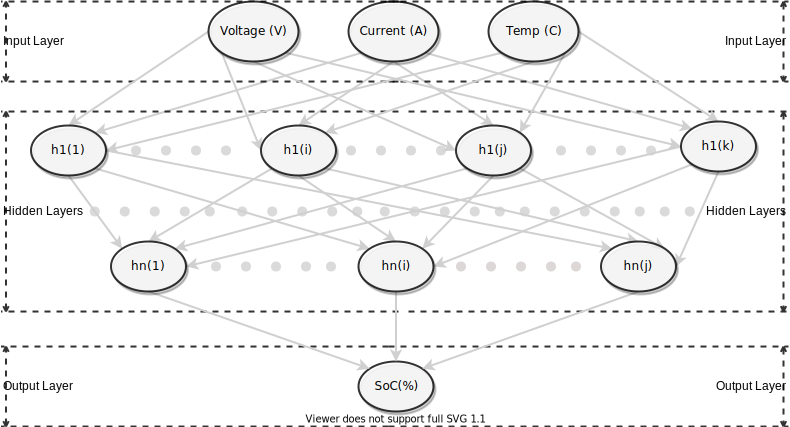
\includegraphics[width=\linewidth]{II_Body/images/SoC-RNN.png}
    \caption{Universal structure of RNN for SoC estimation.}
    \label{fig:RNN-structure}
\end{figure}
\begin{landscape}
    \begin{figure}[ht]
        \centering
        \includegraphics[width=0.9\linewidth]{II_Body/images/Windowing3D-3.jpg}
        \caption{Data Windowing scheme. For visualisation purposes, the $s$-step has been used as 250 seconds, which is different from actual implementation. Initial index $i$ was kept as a value close to the beginning of the data, around zero.}
        \label{fig:Windowing}
    \end{figure}
\end{landscape}
%
%   Model Structure
%
\subsection{Model structure} \label{subsec:structure}
The general summary model structure is represented in Figure~\ref{fig:RNN-structure}, with three feature inputs and a single output.
The number of hidden layers will be dependant on the authors' implementation.
Since the output consists of only a single sample, it is defined by a fully connected layer - a dense layer with a single neuron.
In case if the article did not specify the number of neurons per layer, one of the following equation has been used to get the initial raw estimation~\cite{eckhardt_choosing_2018}:
\begin{equation}
    \begin{split}
        N_h &= \frac{N_s}{ a \left(N_i+N_o \right)} \ \ OR \ \ N_h = \frac{2}{3}\left(N_i+N_o \right) \\
        N_i &\rightarrow \text{Number of input neurons} \\
        N_o &\rightarrow \text{Number of output neurons} \\
        N_s &\rightarrow \text{Number of samples in training data set} \\
        \alpha &\rightarrow \text{An arbitrary scaling factor 2(5)-10}
    \end{split}
\end{equation}
%**Contrary with Hidden Layers as per their name, they obey only internally defined logic and connections.
%**That is why models are stable and reliable once created, cannot be changed, only retrainable with different data.
%A standard Hidden layer, consisting of fully connected neurons, called a Dense Layer.
%A standard Hidden layer, consisting of fully connected neurons and only one or none activation function, called a Dense Layer.
%Within each cell of a Dense layer lies a single activation function.

%An Output Layer gets created from Dense Layer and commonly with no Activation function.
%: \textit{Simple, Exponential or Rectified Linear; Sigmoid and Hyperbolic Tangent functions}. \\
% \begin{itemize}
%     \item \textit{linear} - Simple Linear function
%     \item \textit{elu} - Exponential Linear function
%     \item \textit{relu} - Rectified Linear unit function
%     \item \textit{sigmoind} - Sigmoid function $sigmoid(x) = 1/1(1+exp(-x)$
%     \item \textit{tanh} - Hyperbolic Tangent function $$
% \end{itemize}

%
%
There are several activation functions for those layers widely used in machine learning libraries for time series problems~\cite{amidi_cs_2018}.
For the SoC prediction problem, all authors used the same function.
It also was experimentally confirmed that the best one for all hidden layers is the hyperbolic tangent function, Equation~\ref{eq:tanh}.
The output layer does not use the same logic, and no activation gets applied.
A dropout layer technique with a 20\% cut-off has been applied to all hidden layers to prevent data overfitting over long training periods.
\begin{equation}
    tanh(x) = \frac{sinh(x)}{cosh(x)}=\frac{e^x-e^{-x}}{e^x+e^{-x}}
    \label{eq:tanh}
\end{equation}
%
%
%The common usage of Dense layer in this paper is the Output Layer with no activation functions and with single neuron representing single output SoC value.
%To apply multiple different without overcompicating neurons a multiple bunch of layers with different or the same number of neurons or activations functions gets applied.
%The more Hidden layers network contains - the deeper and computationally complex a network becomes, which also referred as Deep Neural Networks. 

% Choosing the number of neurons for a first Hidden Layer does not have a golden rule.
% For this article, following formula helps to make a good initial estimate based on Number samples, Inout and Output.\\
% \textbf{Equation}\\
% A common practice is to narrow each following Neurons by 2 from previous one, to make a more accurate capture.
% To avoid overfitting data, except for data normalization and Input sample shuffeling in stateles models, a Dropout technue gets applied.
% Tensorflow has an intermnal implementation of Dropoout for GRU and LSTM layers. A value of 0.2 (20\%) applied to all RNN layers to minimizze overfitting possibility.

%
% Requires editing below
The efficiency of an RNN over time series problem is defined by the ability of the neurons to store memory as an internal state.
With time, the memory of long passed samples may fade away.
The problem refereed as vanishing gradient, when the value to update network weights shrinks as it propagates through time~\cite{rasifaghihi_predictive_2020}.
Long-term dependencies do not get captured since layers with a slight gradient do not significantly affect due to insufficient weight change~\cite{rasifaghihi_predictive_2020,hochreiter_vanishing_1998}.
The more complicated structures of neurons tend to solve that problem.
% The gradient is the value used to update Neural Networks’ weight.
%"Therefore, layers that get a small gradient do not learn and they cause the network to have short-term memory."
% https://www.bioinf.jku.at/publications/older/2304.pdf
%"With gradient based learning methods the current error signals has to 'flow back in time' over the feedback connections to past inputs for building up an adequate input storage. Long-term dependancies are hard to learn because of insufficient weight changes."

%
%
There are two commonly used Recurrent Neural Network, which utilises memory cells: Gated Recurrent Unit (GRU) and Long Short-Term Memory (LSTM) with possible extensions implemented by articles' authors.
The GRU implementation will be used as a stateful technique by preserving a state from batch to batch with a single sample at a time.
The LSTM will take a stateless approach, providing a fixed number of timestamps at a time.
%Implementation of the model based on simple RNN using multi layer Dense(X) networks.~\cite{lees2010theoretical}
%A very basic version of Recurrent Neural Network consist of very basic layers with some amount of neurons.

% \subsubsection{Implementation}
%     The input data for a network has been created using Windowing technique, where \textbf{216k} sample of battery data, consisting of State Of Charge only were separated on 500 sample windows.
%     As a results, model outputs a single sample as SoC at next Time Step. Using Tensorflow library and calculating number of Neurons using recomended formula \\
%     \textbf{THIS IS THE BEST PLACE FOR IT}. No other places suites as much.
%     The strcuture of the model ha\subsection{Training and Validation}

%s the following form. (Few Dense Layers+Dropount).
%     A Dropout layer has been used to prevent data overfitting. The selection of activation functions has been done through the properties of the data, which model has to fit in and multiple trials.
% \subsubsection{Observation}
%     A simple Recurrent Neural Network has proven itself effective with simple Linear problems. However, with battery state of charge it is unable to capture complicated features like transition between Discharge and Charge or process of Constant-Voltage Constant-Current charging. In the application of battery utilisation inside Electrical Vehichle, this approach can be used only with some additional logic, such as Kalman Filters.
%     The best approach is to introduce more information about battery state and use more complicated version of Time Series capable to memorise feature with time, such as LSTM~\ref{sec:LSTM} and GRU~\ref{sec:GRU}.
%     The results of the prediction discussed in Section~\ref{sec:results}.
%\subsection{Stateful Gradient Recurrent Unit (GRU) Algorithms and Implementations} \label{subsec:GRU}
%  Gated Recurrent Unit
% Definition of the GRU
%
\subsubsection{Gated Recurrent Unit (GRU) based models} \label{subsub:gru}
One of the methods proposed by Cho et al.~\cite{GRU_cho_properties_2014}, which improves the behaviour of the Neural network, is Gated Recurrent Unit.
Unlike a simple Recurrent NN with a single activation function in the cells, GRU implements different logics to deal with vanishing gradient, as per \mbox{Figure~\ref{fig:GRU-cell}}.
On top of the activation function, it adds two gates related to input and propagated sequences.
The reset gate $r_t$ controls the level information, which has to be ignored.
The update gate $i_t$ controls the impact of previous information on the current status.
The gates implemented by \textit{sigmoid} \mbox{Equation~\ref{eq:sigmoid}} and gated get updated with \mbox{Equations~\ref{eq:GRU-gates}}.
Both gates are related to cell input sequence $x_t$ and the memory cell's output at last time stamp $h_{t-1}$.
%The structure of the layers is similar to a Dense network, with similar input and output layers.
%\textbf{Y. Song~\cite{song_lithium-ion_2018} considered them less complex than another variation (LSTM-RNN) due to the usage of 2 gates rather than 3.}
% \footnote{Bigger value - bigger impact}..
%Weight W and bias b will be the training elements. Bias is added to each gate to increase network flexibility.\\
\begin{figure}[ht]%[htbp]
    \centering
    \includegraphics[width=\linewidth]{II_Body/GRU/images/GRU.jpg}
    \caption{Gated Recurrent Unit Cell}
    \label{fig:GRU-cell}
\end{figure}
\begin{equation}
    \begin{split}
        f_t &= \sigma \left (W_{f} \left [h_{t-1}, x_t \right ] + b_f \right ) \\
        i_t &= \sigma \left (W_{i} \left [h_{t-1}, x_t \right ] + b_i \right )
    \end{split}
    \label{eq:GRU-gates}
\end{equation}
%The standard activation function or content of the memory gets modified with equation~\ref{eq:GRU-output}, where \textit{func} represent the activation function and $\ast$ multiplication by element.
The memory cell output $h_t$ get calculated through the early chosen activation function, $tanh$ in \mbox{Equation~\ref{eq:GRU-output}}.
The $\ast$ stand for multiplication by element.
\begin{equation}
    \begin{split}
        \hat{h_t} &= tanh \left (W_{\hat{h}} \left [f_t \ast h_{t-1}, x_t \right ] + b_{\hat{h}} \right ) \\
        h_t &= \left (1-i_t \right ) h_{t-1}+i_t \hat{h_t}
    \end{split}
    \label{eq:GRU-output}
\end{equation}
% The GRU can act both as a stateful and stateless cell for the model by implementing the model training library.
% For comparison, a Stateful cell will be used per implementation from Song et al.~\cite{song_lithium-ion_2018} and similar articles.
%
% By implementing a model training library, the GRU can act as a stateful and stateless cell for the model.
%(1) - not even count. The method proposed by Y.Song2018, Remaining Useful Life (RUL), \textcolor{red}{uses Capacity only. Nothing more. However, no one mentioned the Statefulnes of GRU models. This would be the best place to introduce it once properly figured out.} \\[2pc]
%
%
% (3) Method proposed by B.Xiao2019 enhances GRU model training with an Ensemble optimisation method.
% Instead of utilising standard Adam optimiser, it combines Nadam and Adamax by running one after another.
% For the first 1/3 training iterations (epochs), Nadam optimiser was used for model pre-training due to its' fast converging speed, then Adamax for model fine-tuning to determine the remaining parameters. \\
% The algorithms for model fitting are as follow \\
%
%
% (8) Similar to LSTM, a Gated Recurrent Unit is intended to solve the vanishing gradient problem.
%     Unlike Chemali2017 implementation, where the training set has consisted of input data sequences with stateles model, BinXio2019 used a stateful model within batches. In addition, it introduced a technique of optimisation to the speedup training process.
%     Implementation of the model based on BinXio or someone else. Introduce their implementation and how to improve optimisation using two algorithms per their discussion.

% \subsection{Implementation}
%     Instead of implementing learning based on Battery Capacity, the following method will use the State of Charge as an input and output, similar to the Dense example. Folowing table highglights parameters, which proven to be most effective during the tests.  \textbf{Table of the parameters like BinXiao}. The activation function was selected as the \textit{tanh} \textbf{the number of sample experementaly was selected as 500?? .} \\
%     \textbf{I have found the place to describe statefulnes for the first time. Potentially, it needs to implement properly. Use the following link to understand how to keep it between batches.}
%https://machinelearningmastery.com/time-series-prediction-lstm-recurrent-neural-networks-python-keras/

 
%\section{GRU with Nadam optimizer}\label{sec:GRU-nadam}
\subsection{Definition}
    Similar to LSTM, a Gradien Recurrent Unit intended to solve problem of vanishing gradient.
    Unlike Chemali2017 implementation, where training set was consisted of input data sequences with stateles model, BinXio2019 used statefull model within batches and intrduced a technique of optimization to speedup training process.
Implementation of the model based on BinXio or someone else. Introduce their way of implementation how to improve optimisation using 2 algorithms as per their discussion.
%\subsection{Stateless Long Short-Term Memory (LSTM) Algorithms and Implementations} \label{subsec:LSTM}
\subsubsection{Long-Short Term Memory based models} \label{subsub:lstm}
The second method and the most commonly used in the Time-series Machine learning model is the Long Short-Term Memory Cell~\cite{LSTM_Hochreiter1997}.
Similar to GRU, LSTM models tend to preserve long-term dependencies in the extended data sequences.
For a longer existence, it became the most widely used type of RNN, used in those types of applications.
Figure~\ref{fig:LSTM-cell} summarises the internal cell logic.
%Currently, the most common usage of the Time-series Machine LEarning model is the prediction of stock prices, weather prognosition or any other time dependant data.
%However, the most common problem for any of those scenarios is vanishing gradient.
%Long range data tend to fade away from the model, which impacts overall prediction.
\begin{figure}[ht]%[htbp]
    \centering
    \includegraphics[width=0.7\linewidth]{II_Body/LSTM/images/LSTM.jpg}
    \caption{Long Short-Term Memory Cell}
    \label{fig:LSTM-cell}
\end{figure}
Unlike GRU, this cell utilises three gates instead of 2.
The update gate gets replaced with separate input $i_t$ and output $o_t$, as per equation~\ref{eq:LSTM-gates}.
All gets utilise the same sigmoid equation~\ref{eq:sigmoid}.
%\textcolor{red}{Those are clasical LSTM approaches. Using history sizes, no Stateless methods.}
%Unlike with GRU, the update gates renamed as an input gate $i_t$, with the same equation. Even that the forget gate $f_t$ is the same, model utilises another one, output gate $g_t$ as per Equations~\ref{eq:LSTM-gates}.
\begin{equation}
    \begin{split}
        f_t &= \sigma \left(W_f \left[h_{t-1}, x_t \right] + b_f \right) \\
        i_t &= \sigma \left(W_i \left[h_{t-1}, x_t \right] + b_i \right) \\
        o_t &= \sigma \left(W_o \left[h_{t-1}, x_t \right] + b_o \right) \\    
    \end{split}
    \label{eq:LSTM-gates}
\end{equation}
The main difference between LSTM and GRU lies in the cell state calculation.
Using the same $tanh$ activation function, Equation~\ref{eq:LSTM-output} describes how cells will be updated and propagated further.
The $c_t$ represents the cell state at a timestamp.
\begin{equation}
    \begin{split}
        \hat{c_t} &= tanh \left(W_c \left[h_{t-1}, x_t \right] + b_c \right) \\
              c_t &= f_t c_{t-1}+i_t \hat{c_t} \\
              h_t &= o_t*tanh \left(c_t \right)II_Body
    \end{split}
    \label{eq:LSTM-output}
\end{equation}
% $c_t \rightarrow$ cell state (memory) at timestep $t$ \\
% $\hat{c_t} \rightarrow$ candidate for cell state \\
% $* \rightarrow$ element wise multiplication \\
Like the GRU cell type, the model training Library supports both stateful and stateless utilisation of the LSTM model.
It will be used as a Stateless cell for further comparison based on Chemali et al.~\cite{Chemali2017} and similar articles.
%
%
% (7) \textcolor{red}{The most complicated one}. Method by WeiZhang2020. Adaptive Time-series prediction on online validation. Data taken directly during cycling batteries.
% \textbf{I have to study this properly first. Long-Horizon, as they called it, more useful ti State if Health. This should be the end of them.}
\subsubsection{Attention Layer}
The research conducted by~\cite{mamo_long_2020} was intended to determine weaknesses and improve the model introducing addition techniques into the default structure of the training model.
They added Attention Layer~\cite{yang_hierarchical_2016} between LSTM and fully connected layers to improve accuracy and replace traditional gradient optimiser with probability-based Differential Evolution.
Figure~\ref{fig:attention} summarises the model structure, and equations~\ref{eq:AttentionWithContext} and~\ref{eq:Addition} define the internal logic between hidden layers and output.

%
%
%bla bla bla... I am exosted, I hgete this part I have no idea what to write and have no desire to research more.
The implementation of the Attention layer does not get provided with the Machine Learning library.
The source code from Winata research~\cite{winata_attention-based_2018} has been used instead.
The open-source code publicly accesses through Github source~\cite{attention_8461990}.
Details in terms of optimiser usage and replacement are justified in subsection~\ref{subsec:optimisers}.
In the State of Charge estimation, the attention layer addresses two shortcomings of LSTM: replacing the traditional method of recursively constructing LSTM depth and located after the output of the primary layer, just before the model Dense layer output~\cite{mamo_long_2020}.
\begin{figure}[htbp]
    \centering
    \includegraphics[width=0.35\linewidth]{II_Body/LSTM/images/AttenrionDrawing.png}
    \caption{Attention based architecture}
    \label{fig:attention}
\end{figure}
\begin{equation}
    \begin{split}
        \hat{u_t} &= tanh \left(W h_{t} + b \right) \\
             \alpha_t &= \frac{exp(u^T u)}{\sum_t(exp(u_t^T u))} \\
              v_t &= \alpha_t*h_t, v in time t
    \end{split}
    \label{eq:AttentionWithContext}
\end{equation}
\begin{equation}
    \begin{split}
        v = \sum_t(\alpha_t * h_t)
    \end{split}
    \label{eq:Addition}
\end{equation}

% \subsection{Implementation}
%     Following table higlighs parameters, which provided best results for their experements.
%     \textbf{Table of the parameters.}
%     The network will be the one discussed above.
%     Model itself will be multi-feature based with follwoing parameters: Voltage \textit{V(t)}, Current \textit{A(t)} and Temperature \textit{C(t)}, where \textit{t} represents a time-stamp. Each feature will contain equal amount of sample and each will be feed in input column vector. As a result, a single input will have following form: \\
%     % [V(0)], [I(0)], [T(0)] \\
%     % [V(1)], [I(1)], [T(1)] \\
%     % [V(n)], [I(n)], [T(n)] \\
%     where \textit{n} is the history size.
%     The output vector will be a State of Charge \textit{SoC(\%)} percentage up to 2 decimal places, within range 0 to 1 and time stamp \textit{n}: \\
%     % [SoC(n)] \\
%     As a result the shape of input and output data will be: X(0)=(n,3) and Y(0)=(1)
%     The entire dataset will use single-step windowing tecnhinue with no bathces to save memory and utilsase \textbf{stateless}* \footnote{Need to discuss this with Holmes.} model. \\
%     The Generated dataset of sample size \textit{k}, will consist of two Tensor input/output Vectors of following shape: \\
%     X = (k-n,n,3), Y = (k-n,1).
%     The variable type for computation was selected to be float32.
%     To keep Denerated dataset simple, no batching approach spared from dealing with 4-dimensional input vectors.
% \subsection{Prediction results}


%     Implementation of the model based on Chemali2017. Application for our section and results. Refer to methodology from time to time.
%\subsection{LSTM with Attention}\label{sec:lstm-attention}
LSTM and GRU models made the most comonly used implemtation of Time -series predictions. TadeleMamo2020 research was intended to determine waknesses and improve the model introducing addition techniques into the default structure of training model***. \\
THe attention mechanissm used in ... \\
THe intention was to capture ... \\
\subsection{Implementation}
    Attention layer implementation was taken from \textbf{refernece} github repositry of ....
    
Implementation of the model based on TadeleMamo 2020 as the most recent and how to implement improvement to the model to make it better. Gracefully transition idea from here to my model, it is similar.
\subsection{Optimisers} \label{subsec:optimisers}
The optimisation algorithm aims to define a way to minimise the difference between model prediction and actual values, using one of the selected Loss functions~\ref{subsub:losses}.
The following section breaks down several methods selected by chosen authors in the growing complexity.
\subsection{Types of optimisers}
The selection of the optimiser defines how fast the model will achieve the local minimum.
Different algorithms utilised several improvements to achieve an optimum result more quickly and avoid overfitting.
All model share the same parameter, the learning rate $\alpha$, which acts as a step to update predictions.
%  Classic Stochastic Gradient Descent
% Explanation
%
\subsubsection{Classic and Momentum Stochastic Gradient Descent Algorithms}
One of the simplest methods to optimise the model is the stochastic gradient descent (SGD), Algorithm~\ref{alg:SGDwM}.
% \begin{algorithm}\captionsetup{labelfont={sc,bf}, labelsep=newline}
%   \caption{Stochastic Gradient Descent (SGD) optimisation}
%   \begin{algorithmic}[1]
%     \STATE \textbf{Number of input samples} \\ $N\gets length(\textit{input data})$\\
%     \STATE \textbf{Size of windows} \\ $S\gets length(V_{i..n})$\\
%     \STATE Input: $x_n = [V_{i..n}, I_{i..n}, T_{i..n}] - $Shape: $X = (N, S, 3)$
%     \STATE Output:$y_n = [SoC_{n}] - $Shape:$Y = (N, 1)$
%     \STATE Define Loss function: $L$ \\
%            Get hyperparameters: $\alpha$
%     \WHILE{$W_t \text{ not converge}$}
%     \STATE $t \gets t+1$
%     \STATE $g_t \gets \nabla_\phi L_t (W_{t-1})$ \COMMENT{Obtain gradient}
%     \STATE $W_t \gets W_{t-1} - \alpha g_t $ \COMMENT{Update parameters}
%     \ENDWHILE
%   \end{algorithmic}
%   \label{alg:SGD}
% \end{algorithm}
The SGD optimiser utilises a simple gradient update with the following learning rate: \mbox{Algorithm~\ref{alg:SGDwM}, Line~\ref{alg:SGDwM-Line-Gradient}}.
% uses fewer calculations and achieves results slower* Higher chances of not achieving the minimum
% Unlike improved versions, this algorithm has the potential of missing optimum value.
The extension of SGD, which Jiao et al.~\cite{jiao_gru-rnn_2020} used, applies a single momentum calculation, \mbox{Algorithm~\ref{alg:SGDwM}, to the classical SGD Line~\ref{alg:SGDwM-Line-Moment}}.
In the text, this is referred to as the stochastic gradient descent with momentum (SGDw/M).
It increases the algorithm's performance by improving the convergence speed compared to the classical~version.
\begin{algorithm}[H]%\captionsetup{labelfont={sc,bf}, labelsep=newline}
  \caption{Stochastic gradient descent with momentum optimisation.}
  \begin{algorithmic}[1]
    \STATE \textbf{Number of input samples} \\ $N\gets length(\textit{input data})$\\
    \STATE \textbf{Size of windows} \\ $S\gets length(V_{i..n})$\\
    \STATE Input: $x_n = [V_{i..n}, I_{i..n}, T_{i..n}] - $Shape: $X = (N, S, 3)$
    \STATE Output:$y_n = [SoC_{n}] - $Shape:$Y = (N, 1)$
    \STATE Define loss function: $L$ \\
    Get hyperparameters: $\alpha, \beta_1$
    \WHILE{$W_t \text{ does not converge}$}
      \STATE $t \gets t+1$
      \STATE $g_t \gets \nabla_W L_t (W_{t-1})$ \COMMENT{obtain gradient \label{alg:SGDwM-Line-Gradient}}
      \STATE $m_t \gets \beta_1 m_{t-1}+(1-\beta_1) g_t $ \COMMENT{1st moment calculation\label{alg:SGDwM-Line-Moment}}
      \STATE $W_t \gets W_{t-1} - \alpha m_t $ \COMMENT{update parameters}
    \ENDWHILE
  \end{algorithmic}
  \label{alg:SGDwM}
\end{algorithm}

% Noising the data
%
% To improve accuracy, Jiao introduced noise to the data to be able to capture more variant information.
% Due to the amount of data provided and comparison with other methods, noise variance will not be used in this implementation.
% \mbox{Table~\ref{tab:params-jiao}} provides parameters selection for the optimiser.
% \begin{table}[ht]
%     \renewcommand{\arraystretch}{1.3}
%     \caption{Hyper-Parameters as per Jiao \textit{et al.}~\cite{jiao_gru-rnn_2020}}
%     \centering
%     \label{tab:params-jiao}
%     \resizebox{\columnwidth}{!}{
%     \begin{tabular}{ l c c }
%       \hline\hline \\[-3mm]
%         Method     & $\alpha$ & $\beta_1 $  \\
%         \hline
%         SGDw/M
%                 & $0.001$ & $0.8$  \\% 0.0000001
%         \hline\hline
%     \end{tabular}
%     }
% \end{table}
% \newpage
\subsubsection{Adam and Robust Online Adam}
The most commonly and by default used in Time-series prediction is Adaptive Moment Estimation~\cite{kingma_adam_2017} (Adam) optimiser.
The algorithm below highlights the steps required to update model weights and bias as per the source.
On top of two constants $\beta$ used for momentum calculation, the algorithm uses $\epsilon$, which referred to as fuzz factor.

%
%
Javid et al.~\cite{javid_adaptive_2020} extended the default $Adam$ algorithm introducing a Robust Online version of Adam, Line 10-12.
Adding the direct influence of loss function to the gradient update adds an online calculation to regular $Adam$ correction.
Table~\ref{tab:adam-params} highlight method-specific parameter selection for the optimiser.
The framework library contained no inbuild implementation of the Robust optimiser.
Instead, it was implemented from the first principal and overwriting the model training procedure.
The code itself can be located in Appendix~\ref{}
\begin{algorithm}\captionsetup{labelfont={sc,bf}, labelsep=newline}
  \caption{Adaptive Moment Estimation (Adam) optimisation}
  \begin{algorithmic}[1]
    \STATE \textbf{Number of input samples} \\ $N\gets length(\textit{input data})$\\
    \STATE \textbf{Size of windows} \\ $S\gets length(V_{i..n})$\\
    \STATE Input: $x_n = [V_{i..n}, I_{i..n}, T_{i..n}] - $Shape: $X = (N, S, 3)$
    \STATE Output:$y_n = [SoC_{n}] - $Shape:$Y = (N, 1)$
    \STATE Define Loss function: $L$ \\
           Get hyperparameters: $\alpha, \beta_1, \beta_2, \epsilon$
    \WHILE{$W_t \text{ not converge}$}
    \STATE $t \gets t+1$
    \STATE $g_t \gets \nabla_W L_t (W_{t-1})$ \COMMENT{Obtain gradient}
    \STATE $m_t \gets \beta_1 m_{t-1}+(1-\beta_1) g_t $ \COMMENT{$1_{st}$ moment calculation}
    \STATE $\upsilon_t \gets \beta_2 \upsilon_{t-1}+ \left(1-\beta_2 \right)g^2_t $ \COMMENT{$2_{nd}$ moment calculation \label{alg:Adam-Line-2Moment}}
    \STATE $\hat{m_t} \gets \frac{m_t}{1-\beta^t_1}$ \COMMENT{Corrected $\hat{m_t}$}
    \STATE $\hat{\upsilon_t} \gets \frac{\upsilon_t}{1-\beta^t_2} $ \COMMENT{Corrected $\hat{\upsilon_t}$}
    \STATE $W_t \gets W_{t-1}- \alpha \frac{\hat{m_t}}{\sqrt{\hat{\upsilon_t}}+\epsilon} $ \COMMENT{Update parameters}
    \ENDWHILE
  \end{algorithmic}
  \label{alg:Adam}
\end{algorithm}
% \begin{tabular}{ l } 
%     \hline
%     Algorithm Adam optimisation  \\
%     \hline
%     %\ \ \textbf{Input:} Data sample with shape=\left(1,500,1,3\right)\\ 
%     %\ \ \textbf{Output:} Predicted SoC shape=\left(1,500,1\right)\\ 
%     \ \ \ 1: Define I/O and Params: $\alpha, \beta_1, \beta_2, \epsilon $ \\
%     \ \ \ 2: Define loss function $L$ \\
%     \ \ \ 3: \textbf{while} $\phi_t$ not converge \textbf{do}: \\
%     \ \ \ 4: \ \ $t \leftarrow t + 1$ \\
%     \ \ \ 5: \ \ $g_t \leftarrow \nabla_\phi L_t \left(\phi_{t-1} \right) $ \text{\ \ \ //Obtain Gradient}\\
%     \ \ \ 6: \ \ $m_t \leftarrow \beta_1 m_{t-1}+ \left(1-\beta_1 \right)g_t $ \text{//$1^{st}$moment }\\
%     \ \ \ 7: \ \ $\upsilon_t\ \leftarrow \beta_2 \upsilon_{t-1}+ \left(1-\beta_2 \right)g^2_t $ \text{//$2^{nd}$moment }\\
%     \ \ \ 8: \ \ $\hat{m_t}\ \ \leftarrow \frac{m_t}{1-\beta^t_1}$ \text{Correct \ \ }$\hat{m_t}$\\
%     \ \ \ 9: \ \ $\hat{\upsilon_t}\ \ \leftarrow \frac{\upsilon_t}{1-\beta^t_2} $ \text{Correct \ \ }$\hat{\upsilon_t}$ \\ \\ \\ \\
%     \ \  10: \ \ $\phi_t \leftarrow \phi_{t-1}- \alpha \frac{\hat{m_t}}{\sqrt{\hat{\upsilon_t}}+\epsilon} $ \\
%     \ \  11: \textbf{end while} \\
%     \hline
% \end{tabular}
\begin{algorithm}\captionsetup{labelfont={sc,bf}, labelsep=newline}
  \caption{Robust Online Adaptive Moment Estimation (Adam) optimisation}
  \begin{algorithmic}[1]
    \STATE \textbf{Number of input samples} \\ $N\gets length(\textit{input data})$\\
    \STATE \textbf{Size of windows} \\ $S\gets length(V_{i..n})$\\
    \STATE Input: $x_n = [V_{i..n}, I_{i..n}, T_{i..n}] - $Shape: $X = (N, S, 3)$
    \STATE Output:$y_n = [SoC_{n}] - $Shape:$Y = (N, 1)$
    \STATE Define Loss function: $L$ \\
           Get hyperparameters: $\alpha, \beta_1, \beta_2, \beta_3, \epsilon$
    \WHILE{$W_t \text{ not converge}$}
    \STATE $t \gets t+1$
    \STATE $g_t \gets \nabla_\phi L_t (W_{t-1})$ \COMMENT{Obtain gradient}
    \STATE $m_t \gets \beta_1 m_{t-1}+(1-\beta_1) g_t $ \COMMENT{$1_{st}$ moment calculation}
    \STATE $\upsilon_t \gets \beta_2 \upsilon_{t-1}+ \left(1-\beta_2 \right)g^2_t $ \COMMENT{$2_{nd}$ moment calculation}
    \STATE $\hat{m_t} \gets \frac{m_t}{1-\beta^t_1}$ \COMMENT{Corrected $\hat{m_t}$}
    \STATE $\hat{\upsilon_t} \gets \frac{\upsilon_t}{1-\beta^t_2} $ \COMMENT{Corrected $\hat{\upsilon_t}$}
    \STATE $r_t \gets \parallel L_t\left(W_{t-1}\right)/L_t\left(W_{t-2}\right) \parallel $ \COMMENT{Relative prediction error term of the loss function}
    \STATE $d_t \gets \beta_3 d_{t-1}+\left(1-\beta_3\right)r_t $ \COMMENT{$3^{rd}$ moment calculation}
    \STATE $W_t \gets W_{t-1}- \alpha \frac{\hat{m_t}}{d_t\sqrt{\hat{\upsilon_t}}+\epsilon} $ \COMMENT{Update parameters}
    \ENDWHILE
  \end{algorithmic}
  \label{alg:RoAdam}
\end{algorithm}
% \begin{tabular}{ l } 
%     \hline
%     Algorithm Robust Adam optimisation  \\
%     \hline
%     %\ \ \textbf{Input:} Data sample with shape=\left(1,500,1,3\right)\\ 
%     %\ \ \textbf{Output:} Predicted SoC shape=\left(1,500,1\right)\\ 
%     \ \ \ 1: Define I/O and Params: $\alpha, \beta_1, \beta_2, \beta_3, \epsilon $ \\
%     \ \ \ 2: Define loss function $L$ \\
%     \ \ \ 3: \textbf{while} $\phi_t$ not converge \textbf{do}: \\
%     \ \ \ 4: \ \ $t \leftarrow t + 1$ \\
%     \ \ \ 5: \ \ $g_t \leftarrow \nabla_\phi L_t\left(\phi_{t-1}\right) $ \\
%     \ \ \ 6: \ \ $m_t \leftarrow \beta_1 m_{t-1}+\left(1-\beta_1\right)g_t $ \\
%     \ \ \ 7: \ \ $\upsilon_t\ \leftarrow \beta_2 \upsilon_{t-1}+\left(1-\beta_2\right)g^2_t $ \\
%     \ \ \ 8: \ \ $\hat{m_t}\ \ \leftarrow \frac{m_t}{1-\beta^t_1}$ \\
%     \ \ \ 9: \ \ $\hat{\upsilon_t}\ \ \leftarrow \frac{\upsilon_t}{1-\beta^t_2} $ \\
%     \ \ \ // Relative prediction error term of the loss function: \\
%     \ \ 10: \ \ $r_t \leftarrow \parallel L_t\left(\phi_{t-1}\right)/L_t\left(\phi_{t-2}\right) \parallel $ \\
%     \ \ 11: \ \ $d_t\ \leftarrow \beta_3 d_{t-1}+\left(1-\beta_3\right)r_t $ \text{//$3^{rd}$moment }\\
%     \ \ 12: \ \ $\phi_t \leftarrow \phi_{t-1}- \alpha \frac{\hat{m_t}}{d_t\sqrt{\hat{\upsilon_t}}+\epsilon} $ \\
%     \ \ 13: \textbf{end while} \\
%     \hline
% \end{tabular}
\begin{table}[htbp]
    \centering
    \caption{Adam, specific parameters}
    \label{tab:adam-params}
    \begin{tabular}{ p{6.0cm} p{1.5cm} p{1.5cm} p{1.5cm} p{1.5cm} p{1.5cm}  }
        \hline
        Source     & $\alpha$ & $\beta_1 $ & $\beta_2$ & $\beta_3$ &  $\epsilon$ \\
        \hline
        Song et al.~\cite{song_lithium-ion_2018} \& Chemale et al.~\cite{Chemali2017}
                & $0.001$ & $0.9$ & $0.999$ & |   &$10^{-8}$ \\% 0.0000001
        Javid et al.~\cite{javid_adaptive_2020}
                & $0.001$ & $0.9$ & $0.999$ & $0.999$ &$10^{-8}$ \\% 0.0000001
        %\hline
        \hline
    \end{tabular}
\end{table}



%  Ensemble optimisation
% Explanation
%
\subsubsection{Ensemble optimisation with Nesterov Momentum Adam and AdaMax}
The Adam algorithm remains the most commonly used optimiser.
The reason behind changing it to another lie in two potential issues.
The first is if the training converges, which may not happen at all~\cite{reddi_convergence_2019}.
The second is if the optimal solution gets frequently missed at large learning steps~\cite{wilson_marginal_2017}.
Xiao \textit{et al.}~\cite{xiao_accurate_2019} proposed a novel alternative of combining several optimisers to address those issues.
The new ensemble optimisation algorithm is based on the combination of Nesterov Momentum Adam (Nadam), \mbox{Algorithm~\ref{alg:nadam}}~\cite{dozat_nadam_2016}, and the AdaMax, \mbox{Algorithm~\ref{alg:adamax}}~\cite{kingma_adam_2017}, at certain moments of training.

% Nadam's advantage over Adam
%
The Nadam optimiser \mbox{Algorithm~\ref{alg:nadam}} extends the Adam, which implements the Nesterov momentum~\cite{dozat_nadam_2016}.
\mbox{Ag~\ref{alg:nadam}, Ln~\ref{alg:Nadam-Line} and Ln~\ref{alg:Nadam-Line-update}} add additional calculations involving gradient and parameters update, intended to improve convergence speed.
% \textcolor{red}{Another error. This time with SQRT. According to Adam and the source code in TF for Nadam, epsilon is not inside sqrt(). Although the original article stands otherwise, Xiao also corrected it. I am sticking with whatever I have at TF. There is no $\beta_i$ and no $\beta_2$ in the second moment update equation. All of that was corrected.}
\begin{algorithm}\captionsetup{labelfont={sc,bf}, labelsep=newline}
    \caption{Nesterov Adaptive Moment Estimation (Nadam) optimisation}
    \begin{algorithmic}[1]
      \STATE \textbf{Number of input samples} \\ $N\gets length(\textit{input data})$\\
      \STATE \textbf{Size of windows} \\ $S\gets length(V_{i..n})$\\
      \STATE Input: $x_n = [V_{i..n}, I_{i..n}, T_{i..n}] - $Shape: $X = (N, S, 3)$
      \STATE Output:$y_n = [SoC_{n}] - $Shape:$Y = (N, 1)$
      \STATE Define Loss function: $L$ \\
             Get hyperparameters: $\alpha, \beta_1, \beta_2, \epsilon$
      \WHILE{$W_t \text{ not converge}$}
      \STATE $t \gets t+1$
      \STATE $g_t \gets \nabla_\phi L_t (W_{t-1})$ \COMMENT{Obtain gradient}
      \STATE $m_t \gets \beta_1 m_{t-1}+(1-\beta_1) g_t $ \COMMENT{$1_{st}$ moment calculation}
      \STATE $\upsilon_t \gets \beta_2 \upsilon_{t-1}+ \left(1-\beta_2 \right)g^2_t $ \COMMENT{$2_{nd}$ moment calculation}
      \STATE $\hat{m_t} \gets \frac{m_t}{1-\beta^t_1}$ \COMMENT{Corrected $\hat{m_t}$}
      \STATE $\hat{\upsilon_t} \gets \frac{\upsilon_t}{1-\beta^t_2} $ \COMMENT{Corrected $\hat{\upsilon_t}$}
      \STATE $\hat{g_t} \gets \frac{g_t}{1-\prod\nolimits_{i = 1}^{k}\beta^t_2} $ \COMMENT{Corrected $\hat{g_t}$\label{alg:Nadam-Line}}
      \STATE $W_t \gets W_{t-1}-\alpha
                          \frac{\left(\beta^{k+1}_1\hat{m_t}+\left(1-\beta^t_1\right)\hat{g_t}\right)}
                               {\sqrt{\hat{\upsilon_t}}+\epsilon}$
                               \COMMENT{Update parameters\label{alg:Nadam-Line-update}}
      % \STATE $W_t \gets W_{t-1}- \alpha \frac{\hat{m_t}}{\sqrt{\hat{\upsilon_t}}+\epsilon} $ // ??
      \ENDWHILE
    \end{algorithmic}
    \label{alg:nadam}
\end{algorithm}

% AdaMax advantages over Adam
%
\mbox{Algorithm~\ref{alg:adamax}} in the ensemble sequence is AdaMax~\cite{kingma_adam_2017}, another modification of the Adam.
The second-order moment on \mbox{Ag~\ref{alg:adamax}, Ln~\ref{alg:AdaMax-Line}} gets replaced with the infinity norm of the moment.
As a result, Xiao \textit{et al.}~\cite{xiao_accurate_2019} considered AdaMax to have a stable weight updating rule and be used in the fine-tuning phase since its' advantage lies in the reduction of gradient fluctuation. 
\begin{algorithm}\captionsetup{labelfont={sc,bf}, labelsep=newline}
    \caption{Adaptive Moment Estimation based on the infinity norm (Adamax)}
    \begin{algorithmic}[1]
      \STATE \textbf{Number of input samples} \\ $N\gets length(\textit{input data})$\\
      \STATE \textbf{Size of windows} \\ $S\gets length(V_{i..n})$\\
      \STATE Input: $x_n = [V_{i..n}, I_{i..n}, T_{i..n}] - $Shape: $X = (N, S, 3)$
      \STATE Output:$y_n = [SoC_{n}] - $Shape:$Y = (N, 1)$
      \STATE Define Loss function: $L$ \\
             Get hyperparameters: $\alpha, \beta_1, \beta_2, \epsilon$
      \WHILE{$W_t \text{ not converge}$}
      \STATE $t \gets t+1$
      \STATE $g_t \gets \nabla_\phi L_t (W_{t-1})$ \COMMENT{Obtain gradient}
      \STATE $m_t \gets \beta_1 m_{t-1}+(1-\beta_1) g_t $ \COMMENT{$1^{st}$ moment calculation}
      \STATE $\upsilon_t \gets max\left(\beta_2\upsilon_{t-1}, |g_t|\right) $ \COMMENT{Corrected $\hat{\upsilon_t}$ \label{alg:AdaMax-Line}}
      % \STATE $W_t \gets W_{t-1}- \alpha \frac{1}{1-\beta^t_1}\frac{m_t}{\upsilon_t} $
      \STATE $W_t \gets W_{t-1}- \alpha \frac{m_t}{(1-\beta^t_1)(\upsilon_t+\epsilon)} $ \COMMENT{Update parameters}
      \ENDWHILE
    \end{algorithmic}
    \label{alg:adamax}
\end{algorithm}

%
%
Xiao \textit{et al.}~\cite{xiao_accurate_2019} considered separating the training process into two stages: pre-training and fine-tuning.
Based on their observations: \textit{``The purpose of the pre-training phase is to endow the GRU model with the appropriate parameters to capture inherent features of the training samples.
The Nadam algorithm uses adaptive learning rates and approximates the gradient using the Nesterov momentum, thereby ensuring fast convergence of the pre-training process."}~\cite[p.~54195]{xiao_accurate_2019}.
The selection of the second algorithm is trivial.
Xiao \textit{et al's}.~\cite{xiao_accurate_2019} selection of AdaMax is defined by fast-convergence to a more stable value for further parameter adjustment.
% \textcolor{red}{I'll be cursed. No, epsilon does. In the TensorFlow implementation, epsilons are added to the vt. Corrected formula added, but commented out. \\
%Remarks made by Xiao justify the usage of the Ensemble algorithm. How would I reprase it into something shorter}\\
%\textit{Remark 1:} The purpose of the pre-training phase os to endow the GRU model with the appropriate parameters to capture the inherent features of the training samples. The Nadam algorithm uses adaptive learning rates and approximates the gradient through the Nesterov momentum, ensuring fast convergence of the pre0training process.
%\textit{Remark 2:} The purpose of the fine-tuning phase is to adjust the parameters further to achieve greater accuracy using the AdaMax algorithm, which converges to a more stable value. \\ \\
The proposed Ensamble algorithm combines both methods for single GRU training, \mbox{Algorithm~\ref{alg:ENS}}.
It describes the adapted version of the Ensemble algorithm, used by the model training procedures, with Nadam for pre-training and AdaMax for fine-tuning phases.
From the results of Xiao \textit{et al.}'s~\cite{xiao_accurate_2019} work $<p_{1}$ and $<p_{2}$ had the same 100 number of epochs.
This scenario will use the value of $<p_{2}$ at the moment the model reaches an overfit with the first phase.
The value of the learning rate will be set to the minimum possible, defined by the research.
\begin{algorithm}\captionsetup{labelfont={sc,bf}, labelsep=newline}
    \caption{Ensemble optimisation training process}
        \begin{algorithmic}[1]
            % \STATE \textbf{Input:} Data sample with shape=(1,500,1,3) 
            % \STATE \textbf{Output:} Predicted SoC shape=(1,1,1)
            \STATE Setup model. Split total number of epoch by 30\% to $p_{1}$ and $p_{2}$ or until model overfits at $p_{2}$
            \STATE Initialise parameters
            \WHILE{epoch  $<p_{1}$:}
                \IF{epoch $<p_{2}$:}
                    \STATE \COMMENT{pass if already compiled with Nadam}
                    \STATE compile model with Nadam parameters. \COMMENT{pre-training phase}
                \ELSE
                    \STATE \COMMENT{pass if already compiled with AdaMax}
                    \STATE compile model with AdaMax parameters. \COMMENT{fine-tuning phase}
                \ENDIF
                \STATE train for a single epoch
            \ENDWHILE
        \end{algorithmic}
    \label{alg:ENS}
\end{algorithm}
%\textcolor{red}{Descibe what shape has been used. Single sample, history length, batch size (if applicable), features number}

%
%
% \mbox{Table~\ref{tab:ensemble-params}} higlights hyper parameters selected by Xiao et al.~\cite{xiao_accurate_2019}.
% \begin{table}[htbp]
%     \renewcommand{\arraystretch}{1.3}
%     \caption{Ensemble, specific parameters}
%     \centering
%     \label{tab:ensemble-params}
%     \resizebox{\columnwidth}{!}{
%     \begin{tabular}{ l c c c c }
%         \hline\hline \\[-3mm]
%         Optimiser     & $\alpha$ & $\beta_1 $ & $\beta_2$ &   $\epsilon$ \\
%         \hline
%         Nadam
%                 & $0.001$ & $0.99$ & $0.999$ & $10^{-8}$ \\% 0.0000001
%         AdaMax
%                 & $5*10^{-4}$ & $0.99$ & $0.999$ & $10^{-8}$ \\% $10^{-8}$
%         \hline
%     \end{tabular}
%     }
% \end{table}


\subsection{Battery Data for training and validation}
Model training has been conducted over Lithium Ion battery cycling data, obtained from CALCE university~\cite{noauthor_calce_2017}.
The SoC value calculated from following equation where $C$ represent Charge and $D$ Discharge Capacities in $Ah$.
Table~\ref{tab:battery} highlights selected battery characteristics.
The Battery Cycling data in a Battery testing chamber were stored as Excel spreadsheets over temperature range 0 and 50 degrees.
Each testing cycle contains 3 testing profiles: Dynamic stress test (DST), (US06) and the Federal urban driving schedule (FUDS).
The temperatrue step 10 degrees with tolerance around 1 degrees.
The range of 20 to 50 was used as training and testing dataset.
Each method went through a single cycling profile and later tested against the other two, as per Mamo \textit{et. al.} \cite{mamo_long_2020} research.
\begin{equation}
    \begin{split}
        \hat{SoC} &= MinMax(C-D) \\
        SoC &= \frac{round(100*\hat{SoC})}{100}
    \end{split}
\end{equation}
\begin{table}[ht]
    \centering
    \caption{Battery characteristics}
    \label{tab:battery}
    \begin{tabular}{ p{2.7cm} p{2.7cm} p{2.7cm} p{2.7cm} p{2.7cm}   }
        \hline
        % \hline
        % \multicolumn{5}{c}{Battery Characteristics} \\
        %\hline
        Brand name & Battery Weight & Nominal  & Nominal & Charge/discharge\\
                   &                & Capacity & Voltage & cut-off voltage \\
        %\hline
        \hline
        %A456 \\ (former A123) & 76g+-1g & 2.3Ah & 3.2V & 3.65V, 2.0 V\\
        A123 (2012) & 76g+-1g & 2.3Ah & 3.2V & 3.65V, 2.0 V\\
        %\hline
        \hline
    \end{tabular}
\end{table}
\subsubsection{Losses}~\label{subsub:losses}
\textcolor{red}{Small description or purpose of the loss functions or what symbol they replace. Redo it to fit whatever I was using.} \\
%\begin{center}
    \begin{tabular}{ l l c }
        \hline
        Name & Articles & Equation \\ 
        \hline
        Absolute Error & Song \textit{et al.}~\cite{song_lithium-ion_2018} & $|SoC_t-\hat{SoC_t}|$ \\
        \hline
        | & Chemal \textit{et al.}\cite{Chemali2017}, Jiao \textit{et al.}~\cite{jiao_gru-rnn_2020} & $\sum\limits^N_{t=0} \frac{1}{2} (SoC_t-\hat{SoC_t})^2$ \\
        \hline
        Mean Average Percentage Error & Mamo \textit{et al.}~\cite{mamo_long_2020} & $\frac{100}{N}\sum\limits^N_{t=0}|\frac{SoC_t-\hat{SoC_t}}{SoC_t}|$ \\
        \hline
        | & Xiao \textit{et al.}~\cite{xiao_accurate_2019} & $\frac{\sum\limits^N_{t=1}(SoC_t-\hat{SoC_t})^2}{N}$ \\
        \hline
        Mean Average Squared Error & Javid \textit{et al.}~\cite{javid_adaptive_2020}, Zhang \textit{et al.}~\cite{zhang_deep_2020} & $\sum\limits^N_{t=0} \sqrt{\frac{1}{n} (SoC_t-\hat{SoC_t})^2}$ \\
        \hline
    \end{tabular}
%\end{center}
\newline
% $ L = \sum\limits^N_{t=0} \frac{1}{2} (SoC_t-\hat{SoC_t})^2$ ~\cite{Chemali2017},~\cite{jiao_gru-rnn_2020} \\
% $ L = \sum\limits^N_{t=0} \sqrt{\frac{1}{n} (SoC_t-\hat{SoC_t})^2}$ ~\cite{javid_adaptive_2020}~\cite{zhang_deep_2020} \\
% $ L = (\sum\limits^N_{t=1}(SoC_t-\hat{SoC_t})^2)N$~\cite{xiao_accurate_2019} \\
% $ L = |SoC_t-\hat{SoC_t}|$ \\
% $ L = \frac{100}{N}\sum\limits^N_{t=0}|\frac{SoC_t-\hat{SoC_t}}{SoC_t}|$~\cite{mamo_long_2020} \\
\subsubsection{Metrics}
\textcolor{red}{Generally, Losses start form 0, metrics from 1. Articles which did overwise were assumed to be mistaken.}
\textcolor{red}{Similar to loses and reasons why we have chosen those as out criterias.} \\
\begin{tabular}{l c}
    \hline
    Mean Average Error &  $\frac{1}{N}\sum\limits^N_{t=1} |SoC_t-\hat{SoC_t}|$ \\
    % \hline
    % Mean Average Percentage Error & $\frac{100}{N}\sum\limits^N_{t=1}|\frac{SoC_t-\hat{SoC_t}}{SoC_t}|$ \\
    \hline
    Root Mean Square Error & $ \sqrt{\frac{1}{N}\sum\limits^N_{t=1} \left(SoC_t-\hat{SoC_t} \right)^2}$ \\
    \hline
    $R^2$ : $M_{SoC}$ is the mean SoC & $1-\frac{\sum\limits^N_{t=1}(SoC_t-\hat{SoC_t})^2}
              {\sum\limits^N_{t=1}(SoC_t-M_{SoC})^2}$ \\
    % \hline
    % Error : Not decided if useful yet & $ \frac{SoC_t-\hat{SoC_5}}{SoC_t}$
\end{tabular}
\\
% $MAE = \frac{1}{N}\sum\limits^N_{t=1} |SoC_t-\hat{SoC_t}|$ \\
% $MAPE = \frac{100}{N}\sum\limits^N_{t=1}|\frac{SoC_t-\hat{SoC_t}}{SoC_t}|$ \\
% $RMSE = \sqrt{\frac{1}{N}\sum\limits^N_{t=1}(SoC_t-\hat{SoC_t})^2}$ \\
% $R^2 = 1-\frac{\sum\limits^N_{t=1}(SoC_t-\hat{SoC_t})^2}
%               {\sum\limits^N_{t=1}(SoC_t-M_{SoC})^2}$ - $M_{SoC}$ is the mean SoC \\
% $Error = \frac{SoC_t-\hat{SoC_5}}{SoC_t}$ - Not decided yet
% \subsubsection{Callbacks}
% For stateless model, the method for reseting a State of model has been derived with Callback function of:
% Another Algorithm. \\
% \begin{lstlisting}[language=Python]
% class ResetCallback(tf.keras.callbacks.Callback):
%     reset_steps : int = 500
%     i_counter   : int = 0
%     def __init__(self):
%         self.i_counter = 0

%     def on_batch_begin(self, batch, logs=None):
%         if (self.i_counter % self.reset_steps) == 0:
%             self.model.reset_states()
%             self.i_counter = 0
%         self.i_counter += 1
% \end{lstlisting}
% \begin{enumerate}
%     \item Checkpoint saving only the best one based on smalest rmse
%     \item Tensorboard tmp folder
%     \item Early stopping is applyable
%     \item Procedure of training epoch by epoch or algorithm for offline and online.
% \end{enumerate}
\subsection{Hardware and Software} \label{subsec:soft}
\textcolor{red}{Need to systemise information better} \\
Tensorflow 2.4.0 with Python 3.9.1 compiled from source with bazel 3.1.0, with packages of Addons version 0.18.* for $R^2$ and Probability 0.* for DE algorithm complied from the source. \\
Attention Layer has been reimpolemented from provided source code.\textcolor{red}{Good luck finding the link}
Tensorboard used to observe progress as it goes and keep records to analyze training later.
Hardware Intel CPU with Graphical Processor with Compute Capability Score of 7.5, CUDA version 11.1.
Multilayer model flaged with Return sequences boolean. Statefulnes define with Stateful boolean. The dropout affected as separate layer or parameter. With Stateful on, standard Inpust Layer shape requires to be follower Bacthed Input shape. It can be done kwarg parameter to the GRU or LSTM layer or kept as a separate Input Layer to allow precompilation before starting model fitting. Following code snipest demonstrated the difference. \\
\textcolor{red}{I am going to use the TPU processor to measure time it takes to run each model.} \\
\begin{table}[ht]
    \centering
    \caption{Software details}
    \label{tab:my_label}
    \begin{tabular}{p{3.0cm}|c|c|c|c|c}
        Version & Python version & Compiler & Build tools & CUDA version & Compute Score\\
        Tensorflow-2.4.0, TF-Addons 13.0, TF-Probability 0.12.1 & 3.9.1 & gcc 9.3.0 & Bazel 3.1.0 & 11.1 & 7.5\\
        \hline
        Tensorflow-2.2.0 & 3.8.* & gcc 7.3.1 & Bazel 2.0.0 & CPU & 3.98MHz*
    \end{tabular}
\end{table}
\begin{table}[]
    \centering
    \caption{Chip-on-Board Hardware selection}
    \label{tab:my_label}
    \begin{tabular}{c|c|c|c}
        Device & Specification & Source & Software setup \\
        \hline
        Coral TPU & (Specs) & (Link to the details) & (Link to libedgetpu.so.1) \\
        \hline
        Raspberry Pi 4 (Active cooling) & 
    \end{tabular}
\end{table}